% Options for packages loaded elsewhere
\PassOptionsToPackage{unicode}{hyperref}
\PassOptionsToPackage{hyphens}{url}
\PassOptionsToPackage{dvipsnames,svgnames,x11names}{xcolor}
%
\documentclass[
  letterpaper,
  DIV=11,
  numbers=noendperiod]{scrartcl}

\usepackage{amsmath,amssymb}
\usepackage{iftex}
\ifPDFTeX
  \usepackage[T1]{fontenc}
  \usepackage[utf8]{inputenc}
  \usepackage{textcomp} % provide euro and other symbols
\else % if luatex or xetex
  \usepackage{unicode-math}
  \defaultfontfeatures{Scale=MatchLowercase}
  \defaultfontfeatures[\rmfamily]{Ligatures=TeX,Scale=1}
\fi
\usepackage{lmodern}
\ifPDFTeX\else  
    % xetex/luatex font selection
\fi
% Use upquote if available, for straight quotes in verbatim environments
\IfFileExists{upquote.sty}{\usepackage{upquote}}{}
\IfFileExists{microtype.sty}{% use microtype if available
  \usepackage[]{microtype}
  \UseMicrotypeSet[protrusion]{basicmath} % disable protrusion for tt fonts
}{}
\makeatletter
\@ifundefined{KOMAClassName}{% if non-KOMA class
  \IfFileExists{parskip.sty}{%
    \usepackage{parskip}
  }{% else
    \setlength{\parindent}{0pt}
    \setlength{\parskip}{6pt plus 2pt minus 1pt}}
}{% if KOMA class
  \KOMAoptions{parskip=half}}
\makeatother
\usepackage{xcolor}
\setlength{\emergencystretch}{3em} % prevent overfull lines
\setcounter{secnumdepth}{-\maxdimen} % remove section numbering
% Make \paragraph and \subparagraph free-standing
\makeatletter
\ifx\paragraph\undefined\else
  \let\oldparagraph\paragraph
  \renewcommand{\paragraph}{
    \@ifstar
      \xxxParagraphStar
      \xxxParagraphNoStar
  }
  \newcommand{\xxxParagraphStar}[1]{\oldparagraph*{#1}\mbox{}}
  \newcommand{\xxxParagraphNoStar}[1]{\oldparagraph{#1}\mbox{}}
\fi
\ifx\subparagraph\undefined\else
  \let\oldsubparagraph\subparagraph
  \renewcommand{\subparagraph}{
    \@ifstar
      \xxxSubParagraphStar
      \xxxSubParagraphNoStar
  }
  \newcommand{\xxxSubParagraphStar}[1]{\oldsubparagraph*{#1}\mbox{}}
  \newcommand{\xxxSubParagraphNoStar}[1]{\oldsubparagraph{#1}\mbox{}}
\fi
\makeatother


\providecommand{\tightlist}{%
  \setlength{\itemsep}{0pt}\setlength{\parskip}{0pt}}\usepackage{longtable,booktabs,array}
\usepackage{calc} % for calculating minipage widths
% Correct order of tables after \paragraph or \subparagraph
\usepackage{etoolbox}
\makeatletter
\patchcmd\longtable{\par}{\if@noskipsec\mbox{}\fi\par}{}{}
\makeatother
% Allow footnotes in longtable head/foot
\IfFileExists{footnotehyper.sty}{\usepackage{footnotehyper}}{\usepackage{footnote}}
\makesavenoteenv{longtable}
\usepackage{graphicx}
\makeatletter
\newsavebox\pandoc@box
\newcommand*\pandocbounded[1]{% scales image to fit in text height/width
  \sbox\pandoc@box{#1}%
  \Gscale@div\@tempa{\textheight}{\dimexpr\ht\pandoc@box+\dp\pandoc@box\relax}%
  \Gscale@div\@tempb{\linewidth}{\wd\pandoc@box}%
  \ifdim\@tempb\p@<\@tempa\p@\let\@tempa\@tempb\fi% select the smaller of both
  \ifdim\@tempa\p@<\p@\scalebox{\@tempa}{\usebox\pandoc@box}%
  \else\usebox{\pandoc@box}%
  \fi%
}
% Set default figure placement to htbp
\def\fps@figure{htbp}
\makeatother
% definitions for citeproc citations
\NewDocumentCommand\citeproctext{}{}
\NewDocumentCommand\citeproc{mm}{%
  \begingroup\def\citeproctext{#2}\cite{#1}\endgroup}
\makeatletter
 % allow citations to break across lines
 \let\@cite@ofmt\@firstofone
 % avoid brackets around text for \cite:
 \def\@biblabel#1{}
 \def\@cite#1#2{{#1\if@tempswa , #2\fi}}
\makeatother
\newlength{\cslhangindent}
\setlength{\cslhangindent}{1.5em}
\newlength{\csllabelwidth}
\setlength{\csllabelwidth}{3em}
\newenvironment{CSLReferences}[2] % #1 hanging-indent, #2 entry-spacing
 {\begin{list}{}{%
  \setlength{\itemindent}{0pt}
  \setlength{\leftmargin}{0pt}
  \setlength{\parsep}{0pt}
  % turn on hanging indent if param 1 is 1
  \ifodd #1
   \setlength{\leftmargin}{\cslhangindent}
   \setlength{\itemindent}{-1\cslhangindent}
  \fi
  % set entry spacing
  \setlength{\itemsep}{#2\baselineskip}}}
 {\end{list}}
\usepackage{calc}
\newcommand{\CSLBlock}[1]{\hfill\break\parbox[t]{\linewidth}{\strut\ignorespaces#1\strut}}
\newcommand{\CSLLeftMargin}[1]{\parbox[t]{\csllabelwidth}{\strut#1\strut}}
\newcommand{\CSLRightInline}[1]{\parbox[t]{\linewidth - \csllabelwidth}{\strut#1\strut}}
\newcommand{\CSLIndent}[1]{\hspace{\cslhangindent}#1}

\usepackage{booktabs}
\usepackage{longtable}
\usepackage{array}
\usepackage{multirow}
\usepackage{wrapfig}
\usepackage{float}
\usepackage{colortbl}
\usepackage{pdflscape}
\usepackage{tabu}
\usepackage{threeparttable}
\usepackage{threeparttablex}
\usepackage[normalem]{ulem}
\usepackage{makecell}
\usepackage{xcolor}
\KOMAoption{captions}{tableheading}
\makeatletter
\@ifpackageloaded{caption}{}{\usepackage{caption}}
\AtBeginDocument{%
\ifdefined\contentsname
  \renewcommand*\contentsname{Table of contents}
\else
  \newcommand\contentsname{Table of contents}
\fi
\ifdefined\listfigurename
  \renewcommand*\listfigurename{List of Figures}
\else
  \newcommand\listfigurename{List of Figures}
\fi
\ifdefined\listtablename
  \renewcommand*\listtablename{List of Tables}
\else
  \newcommand\listtablename{List of Tables}
\fi
\ifdefined\figurename
  \renewcommand*\figurename{Figure}
\else
  \newcommand\figurename{Figure}
\fi
\ifdefined\tablename
  \renewcommand*\tablename{Table}
\else
  \newcommand\tablename{Table}
\fi
}
\@ifpackageloaded{float}{}{\usepackage{float}}
\floatstyle{ruled}
\@ifundefined{c@chapter}{\newfloat{codelisting}{h}{lop}}{\newfloat{codelisting}{h}{lop}[chapter]}
\floatname{codelisting}{Listing}
\newcommand*\listoflistings{\listof{codelisting}{List of Listings}}
\makeatother
\makeatletter
\makeatother
\makeatletter
\@ifpackageloaded{caption}{}{\usepackage{caption}}
\@ifpackageloaded{subcaption}{}{\usepackage{subcaption}}
\makeatother

\usepackage{bookmark}

\IfFileExists{xurl.sty}{\usepackage{xurl}}{} % add URL line breaks if available
\urlstyle{same} % disable monospaced font for URLs
\hypersetup{
  pdftitle={Pre-Columbian forest gardens span 180 km² in Bolivia's Iténez preserve},
  colorlinks=true,
  linkcolor={blue},
  filecolor={Maroon},
  citecolor={Blue},
  urlcolor={Blue},
  pdfcreator={LaTeX via pandoc}}


\title{Pre-Columbian forest gardens span 180 km² in Bolivia's Iténez
preserve}
\author{Nicolas Gauthier}
\date{}

\begin{document}
\maketitle
\begin{abstract}
The Iténez Forest Preserve in the Bolivian Amazon spans 4,000 km²
between two of South America's most significant archaeological
landscapes---yet until now it remained unmapped, a blank spot between
lowland Bolivia and the Brazilian Amazon. Using satellite imagery from
the driest months on record and an AI-assisted detection system, I
identified 180 km² of anthropogenic soils and forest gardens across the
preserve. These features, connected by dense networks of earthworks that
remain to be fully mapped, reveal organized landscape modification on a
scale comparable to the region's famous earthwork complexes. The
findings demonstrate how ancient peoples transformed rainforest into
productive cultural landscapes whose ecological signatures persist
today, with local communities continuing to harvest cacao and other
useful species from these anthropogenic forests. This work illustrates
how AI can support---but not replace---human expertise in archaeological
detection at regional scales.
\end{abstract}


\textsubscript{Source:
\href{https://nick-gauthier.github.io/itenez-forest-gardens/index-preview.html}{Article
Notebook}}

\subsection{Introduction}\label{introduction}

For decades, a 4,000 km² void has persisted in archaeological maps of
the Amazon, separating the well-studied earthwork landscapes of Bolivia
from the forests of the Brazilian Amazon. The Iténez Forest Preserve
occupies this glaring gap along the Bolivia-Brazil border. Located along
the Bolivia-Brazil border between the extensively studied earthwork
landscapes of the Bolivian lowlands and the forests of the Brazilian
Amazon, this 4,000 km² expanse of forest remained largely unmapped by
archaeologists. While important studies have documented sites at the
preserve's northern and southern margins (Robinson et al. 2021; Prümers,
Jaimes Betancourt, and Plaza Martinez 2023; Carson et al. 2016) , the
rugged interior---the vast majority of this territory---has remained
archaeologically unknown. Dense canopy cover, remoteness, and lack of
prior survey work in the interior left it a blank spot on regional
maps---a void in our understanding of southwestern Amazonian prehistory.
Its position between known centers of pre-Columbian engineering
(Peripato et al. 2023; De Souza et al. 2018), however, suggested it
might hold similar evidence of ancient landscape modification.

This study fills that gap through systematic remote sensing analysis,
revealing extensive anthropogenic landscapes hidden beneath the forest
canopy. The work focuses specifically on detecting Amazonian Dark Earth
(ADE) and associated forest gardens---patches of modified forest
composition that mark ancient settlements and agricultural areas
(Schmidt et al. 2014; Palace et al. 2017; Goldberg et al. 2024) . While
earthworks are noted where visible, comprehensive mapping of these
features beneath the canopy remains for future work. This approach
prioritizes the detection of anthropogenic soils and forest composition
changes that represent the primary evidence of human landscape
transformation in continuously forested regions.

\begin{figure}[H]

{\centering \pandocbounded{\includegraphics[keepaspectratio]{images/clipboard-2087942158.jpeg}}

}

\caption{Sentinel-2 false color image composite of Itenez Forest
Preserve from summer 2023. Light red spots indicate drier , lowcanopy
vegetation associated with anthropogenic forest gardens (palms, cacao,
bamboo, and other economically useful plants).}

\end{figure}%

The detection of these features at regional scale required developing
new methodological approaches that combine AI-assisted pattern
recognition with expert archaeological interpretation---a partnership
where computational tools support but do not replace human expertise in
identifying and mapping cultural landscapes.

\subsection{Methods}\label{methods}

\subsubsection{Image Selection and
Processing}\label{image-selection-and-processing}

I selected Sentinel-2 imagery (European Union/ESA/Copernicus 2017) from
the driest periods in the satellite record (late summer 2023 and 2024),
when reduced vegetation moisture and seasonal leaf loss maximize
visibility of underlying soil and vegetation patterns. Cloud-free
mosaics were processed in Google Earth Engine, combined with a state of
the art regional canopy height model (Wagner et al. 2025) to distinguish
anthropogenic forest structures from natural variation.

\begin{figure}[H]

{\centering \pandocbounded{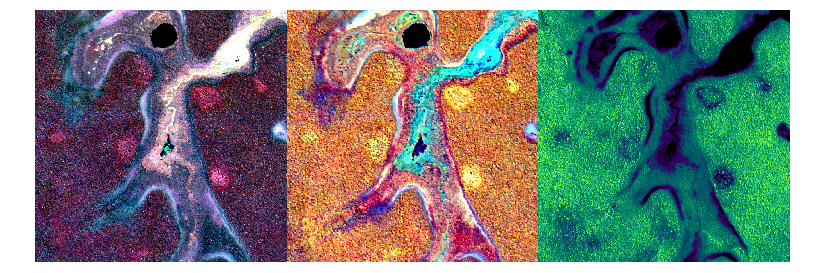
\includegraphics[keepaspectratio]{index_files/figure-pdf/unnamed-chunk-1-1.pdf}}

}

\caption{False color Sentinel 2 image chips (left, center) and canopy
height estimate (right). Anthropogenic forest patches appears as rounded
patches of dry, low-canopy vegetation along terraces. Faint traces of
earthworks and ditches can be seen surrounding and connecting the forest
patches.}

\end{figure}%

\textsubscript{Source:
\href{https://nick-gauthier.github.io/itenez-forest-gardens/index-preview.html}{Article
Notebook}}

The imagery was exported as multi-scale tiles (512, 768, and 1024
pixels) with band combinations optimized to highlight spectral
signatures of ADE and modified forest. These signatures reflect the
distinct ecological characteristics of anthropogenic landscapes: more
open canopy structure, seasonal deciduousness, high concentrations of
useful plants (palms, bamboos, cacao), and altered soil chemistry from
centuries of human occupation and management Robinson et al. (2021).

\begin{figure}[H]

{\centering \pandocbounded{\includegraphics[keepaspectratio]{images/clipboard-593555342.png}}

}

\caption{Detail of transition between natural forest vegetation (left)
and anthropogenic forest (right). Not the lighter vegetation, lower
canopy, and preponderance of palms and lianas.}

\end{figure}%

\subsubsection{Detection Workflow: Human-AI
Partnership}\label{detection-workflow-human-ai-partnership}

I developed an agentic object detection system using GPT-4.1, and
Moondream2 vision-language models to identify anthropogenic features at
scale. This system serves as a detection and verification tool,
supporting human expertise rather than replacing it. The workflow
operates as follows:

\begin{enumerate}
\def\labelenumi{\arabic{enumi}.}
\tightlist
\item
  GPT models review imagery and generate initial hypotheses about
  feature locations based on spectral patterns and landscape context.
  They are prompted to view the landscape holistically, looking for
  patterns across multiple domains, rather than focusing on strict
  quantitative criteria.
\item
  The primary models iteratively refine predictions through successive
  passes using a smaller, specialized vision language models tuned for
  object detection and grounding. These system lack the domain knowledge
  of the image contents, so the GPT agent must generate creative,
  abstract text prompts to detect all features in the scene
  (e.g.~``reddish-pink spots'', ``purple swirls''.
\item
  The system produces point predictions marking potential anthropogenic
  sites
\item
  These points guide large-scale verification and exploration of spatial
  patterns
\end{enumerate}

\textbf{Examples:}

\pandocbounded{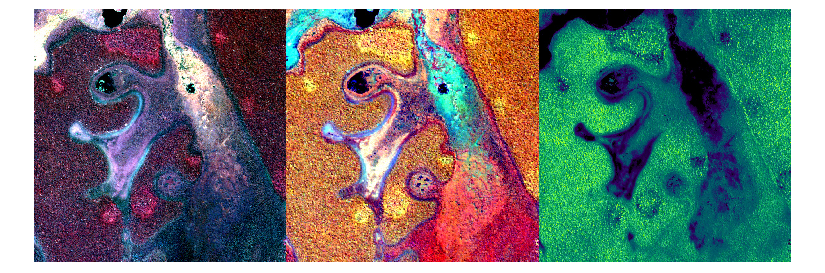
\includegraphics[keepaspectratio]{index_files/figure-pdf/unnamed-chunk-2-1.pdf}}

\textsubscript{Source:
\href{https://nick-gauthier.github.io/itenez-forest-gardens/index-preview.html}{Article
Notebook}}

\begin{verbatim}
**Scene interpretation (Step 1):**

- **C1:** Shows several compact, lobate, and elliptical reddish-pink/magenta 
patches, especially in the lower left, lower center, and upper left. These are 
embedded within a mottled forest matrix, not at a forest/nonforest boundary. 
Some patches have faint linear connections or ring-like forms.
- **C2:** The same areas show strong yellow/orange signals, supporting the 
presence of stressed/drier vegetation typical of ADE patches. The yellow/orange
is compact and matches the C1 anomalies.
- **CHM:** These patches correspond to areas of lower canopy height (darker 
blue/purple), sometimes with a ring or edge effect, further supporting the 
interpretation as ADE patches.

**Spatial context:** The anomalies are compact, not diffuse, and are located 
within continuous forest, not at the edge or in floodplain. Some are clustered 
or show faint linear/ring connections, consistent with anthropogenic earthwork 
patterns.

**Initial expert estimate:** There are at least 3–4 distinct, compact ADE-like 
patches in this scene, possibly up to 5 depending on how the lobate forms are 
counted.

**Proceeding to Moondream object detection (Step 2).**

**First tool prompts:**
- "reddish-pink spots"
- "magenta patches"

Running these in parallel to capture the main compact anomalies.
\end{verbatim}

\begin{verbatim}
**Synthesis (Step 3):**

- Both prompts ("reddish-pink spots", "magenta patches") returned highly 
overlapping sets of points, confirming the main compact anomalies.
- After removing duplicates, there are 7 unique candidate patches:
  1. (0.0918, 0.2998) – Lower left, compact, strong spectral/structural 
support.
  2. (0.292, 0.8223) – Lower center, compact, strong support.
  3. (0.4375, 0.7656) – Lower center-right, compact, strong support.
  4. (0.6309, 0.5967) – Center-right, compact, strong support.
  5. (0.7344, 0.1084) – Upper right, compact, strong support.
  6. (0.8486, 0.3789) – Right edge, compact, strong support.
  7. (0.9678, 0.6709) – Far right edge, compact, but needs context check.

- All points correspond to compact, lobate, or elliptical reddish/magenta 
patches in C1, with matching yellow/orange in C2 and low canopy in CHM.
- All are within continuous forest, not at a forest/nonforest boundary.
- The far right edge point (0.9678, 0.6709) is at the image margin but fits the
broader spatial pattern.

**Summary of synthesis:**
- 7 distinct, compact ADE-like patches detected.
- All have dual spectral support, compact form, and context fit.
- No diffuse or nonforest-edge anomalies included.
- Detections are consistent with ancient anthropogenic ADE/earthwork patterns.

DONE.
\end{verbatim}

\textsubscript{Source:
\href{https://nick-gauthier.github.io/itenez-forest-gardens/index-preview.html}{Article
Notebook}}

\pandocbounded{\includegraphics[keepaspectratio]{index_files/figure-pdf/unnamed-chunk-4-1.pdf}}

\textsubscript{Source:
\href{https://nick-gauthier.github.io/itenez-forest-gardens/index-preview.html}{Article
Notebook}}

\pandocbounded{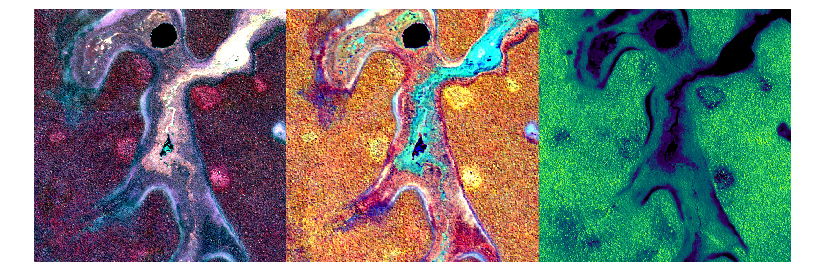
\includegraphics[keepaspectratio]{index_files/figure-pdf/unnamed-chunk-5-1.pdf}}

\textsubscript{Source:
\href{https://nick-gauthier.github.io/itenez-forest-gardens/index-preview.html}{Article
Notebook}}

\begin{verbatim}
**Scene interpretation (Step 1):**

- **C1:** Several compact, lobate reddish-pink/magenta patches are visible, 
especially to the right of the main drainage, and a few to the left. These are 
embedded within a mottled forest matrix, not at the forest edge or in 
open/floodplain areas. The patches are distinct, not diffuse, and have 
plausible ADE-like form and size (≥5 ha).
- **C2:** These same areas correspond to bright yellow/orange splotches, 
supporting the interpretation of stressed/drier vegetation typical of ADE 
patches.
- **CHM:** The candidate patches show subtle but consistent lower canopy height
(darker blue/purple) compared to the surrounding matrix, sometimes with a 
ringed or compact form.

**Context:** The anomalies are located on a bluff above a drainage, not on the 
floodplain, and are not simply forest islands. There are at least 3–5 plausible
ADE patch candidates, with some spatial patterning.

**Initial expert estimate:** 4–5 compact ADE-like patches.

Proceeding to Moondream object detection for precise locations.
\end{verbatim}

\begin{verbatim}
**Synthesis of Moondream points (Step 3):**

- All three prompts ("reddish-pink spots", "magenta patches", "lobate red 
blobs") returned highly consistent sets of points, with only minor coordinate 
variation.
- After removing duplicates and checking against the imagery:
  - 5 compact, plausible ADE patch candidates are confirmed. These are all 
within the continuous forest matrix, have strong dual spectral support (C1/C2),
and show subtle but consistent CHM anomalies (lower canopy).
  - Two additional points (lower left and lower right edge) are at/near the 
image edge but are consistent with the broader spatial pattern and context.
  - All detected patches are ≥5 ha and have compact, lobate/elliptical form.

**Summary:** 5–6 distinct ADE-like patches, all with strong spectral-structural
support and appropriate context. Will finalize and deduplicate for the final 
result.

DONE.
\end{verbatim}

\textsubscript{Source:
\href{https://nick-gauthier.github.io/itenez-forest-gardens/index-preview.html}{Article
Notebook}}

\pandocbounded{\includegraphics[keepaspectratio]{index_files/figure-pdf/unnamed-chunk-7-1.pdf}}

\textsubscript{Source:
\href{https://nick-gauthier.github.io/itenez-forest-gardens/index-preview.html}{Article
Notebook}}

\pandocbounded{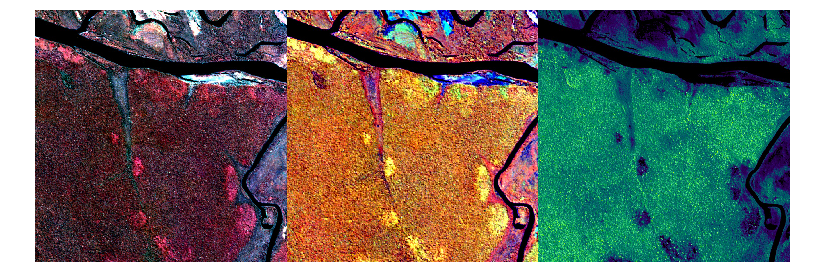
\includegraphics[keepaspectratio]{index_files/figure-pdf/unnamed-chunk-8-1.pdf}}

\textsubscript{Source:
\href{https://nick-gauthier.github.io/itenez-forest-gardens/index-preview.html}{Article
Notebook}}

\begin{verbatim}
**Scene interpretation (Step 1):**

- **C1:** Several compact, lobate, reddish-pink/magenta patches are visible, 
especially in the central and lower portions of the image. These patches are 
distinct from the surrounding forest matrix, which is more mottled and darker. 
The patches are not diffuse, and some appear loosely clustered or aligned along
subtle linear features.
- **C2:** The same areas show strong yellow/orange splotches, confirming low 
transpiration and supporting the presence of stressed/dry vegetation typical of
ADE patches.
- **CHM:** These patches correspond to areas of slightly lower canopy height 
(darker blue/purple), sometimes with a ring or core structure, further 
supporting the interpretation as ADE forest patches.

**Context:** The anomalies are within a continuous forest matrix, not at the 
forest edge or in floodplain, and are compact, not diffuse. Some are loosely 
aligned along subtle drainage or earthwork traces.

**Initial expert estimate:** There are approximately 7–9 valid ADE patch 
candidates in this scene.

Proceeding to Moondream object detection for precise point locations.
\end{verbatim}

\begin{verbatim}
**Synthesis of Moondream results (Step 3):**

- Both prompts ("reddish-pink spots", "large magenta patches") returned 
overlapping sets of points, with strong clustering in the central, lower, and 
right-central portions of the image.
- After removing redundant/overlapping points and excluding those that are too 
small, at the image edge, or lack compactness/context, I identify 8 distinct, 
compact ADE patch candidates:
  - Central vertical cluster (3): (0.4102, 0.6172), (0.4102, 0.8301), (0.5, 
0.9248)
  - Lower right cluster (3): (0.7783, 0.71), (0.834, 0.834), (0.832, 0.6006)
  - Right-central (1): (0.8564, 0.335)
  - Central left (1): (0.3193, 0.5068)
- All selected points have strong dual spectral support (C1/C2), compact form, 
and context fit (within continuous forest, not at edge or in floodplain).
- Some additional points (e.g., at extreme top/left edges) are excluded due to 
insufficient context or size.

**Summary:** 8 distinct ADE patch candidates identified, all with strong 
spectral, structural, and contextual support.

DONE.
\end{verbatim}

\textsubscript{Source:
\href{https://nick-gauthier.github.io/itenez-forest-gardens/index-preview.html}{Article
Notebook}}

\pandocbounded{\includegraphics[keepaspectratio]{index_files/figure-pdf/unnamed-chunk-10-1.pdf}}

\textsubscript{Source:
\href{https://nick-gauthier.github.io/itenez-forest-gardens/index-preview.html}{Article
Notebook}}

Critically, this AI component operated in parallel with detailed manual
mapping. I meticulously reviewed and labeled hundreds of polygon
boundaries over anthropogenic forest patches through careful imagery
analysis, with the AI and manual mapping developing iteratively and
informing each other. Earthworks---canals, ditches, and geometric
earthworks---were recorded where visible through the canopy, though
comprehensive mapping of these linear features remains a priority for
future work with higher-resolution imagery. This approach allowed me to
iteratively calibrate and validate the models' ability to detect known
archaeological features in zero-shot and few-shot learning contexts. The
models were not fine-tuned but leveraged pre-trained capabilities to
recognize visual patterns consistent with archaeological features. This
approach exemplifies how AI can extend human capacity for regional-scale
analysis without replacing the expertise necessary for accurate feature
identification and interpretation.

\subsection{Results}\label{results}

The analysis \textbf{identified approximately 180 km² of anthropogenic
soils and forest gardens within the Iténez Forest Preserve, representing
5\% of its total area---comparable to the footprint of many modern world
cities}, though distributed as a network of patches rather than a
contiguous area. I mapped over 350 individual fields ranging from 5 to
700 hectares, with clear spatial clustering along bluffs, drainages, and
floodplain margins in upland \emph{terra firme} forest---confirming
hypotheses about bluff-edge settlement systems previously proposed for
this region (Denevan 1996).

\begin{figure}[H]

{\centering \pandocbounded{\includegraphics[keepaspectratio]{index_files/figure-pdf/unnamed-chunk-11-1.pdf}}

}

\caption{Anthropogenic forest patches.}

\end{figure}%

\begin{verbatim}

|---------|---------|---------|---------|
=========================================
                                          
\end{verbatim}

\begin{figure}[H]

{\centering \pandocbounded{\includegraphics[keepaspectratio]{index_files/figure-pdf/unnamed-chunk-11-2.pdf}}

}

\caption{Anthropogenic forest patches.}

\end{figure}%

\textsubscript{Source:
\href{https://nick-gauthier.github.io/itenez-forest-gardens/index-preview.html}{Article
Notebook}}

\begin{figure}[H]

{\centering \pandocbounded{\includegraphics[keepaspectratio]{index_files/figure-pdf/unnamed-chunk-12-1.pdf}}

}

\caption{Manually labeled site locations (black) compared to
automatically detected locations (red).}

\end{figure}%

\textsubscript{Source:
\href{https://nick-gauthier.github.io/itenez-forest-gardens/index-preview.html}{Article
Notebook}}

The most striking discovery is a major complex spanning more than 4
kilometers, where large-scale fields connect through networks of
earthworks. Across the mapped area, an exceptionally dense system of
linear features links settlements into an integrated landscape. While
full mapping of these earthworks awaits future work with
canopy-penetrating sensors, their visible portions already demonstrate a
level of landscape integration comparable to the most complex sites in
neighboring regions.

\pandocbounded{\includegraphics[keepaspectratio]{images/clipboard-4170918036.jpeg}}

Rank-size analysis reveals a clear hierarchical structure in field sizes
and site distribution, with the size distribution following a power law
with an exponent close to 1 on log-log plots. This pattern, consistent
with organized settlement systems, matches the scale and complexity
documented in the Llanos de Mojos and Baures (Prümers et al. 2022;
Erickson 2000). The largest sites anchor networks of settlement and
agroforestry patches, suggesting centralized planning and resource
management across the landscape.

\pandocbounded{\includegraphics[keepaspectratio]{index_files/figure-pdf/unnamed-chunk-13-1.pdf}}

\textsubscript{Source:
\href{https://nick-gauthier.github.io/itenez-forest-gardens/index-preview.html}{Article
Notebook}}

These anthropogenic landscapes remain ecologically distinct today.
Forest composition in mapped areas shows high concentrations of
economically useful species, particularly cacao, making the region a
modern hotspot for wild cacao cultivation---a direct legacy of ancient
land use practices (Carson et al. 2016) . Local and Indigenous
communities continue to harvest these resources, underscoring that these
are not merely archaeological sites but living landscapes where ancient
management practices continue to shape both forest ecology and human
livelihoods.

\subsection{Discussion}\label{discussion}

These findings transform our understanding of the Iténez region from
archaeological blank spot to critical piece in the Amazonian puzzle. The
extent and organization of anthropogenic landscapes documented here
match or exceed those in better-studied areas, confirming that
large-scale landscape engineering extended continuously across the
southwestern Amazon. This fills the last major gap in the regional
archaeological map between the Llanos de Mojos and Baures, revealing
that the Iténez was not a periphery but an integral part of
pre-Columbian regional systems.

The hierarchical site structure and extensive earthwork networks point
to complex social organization capable of coordinating landscape
modification across thousands of square kilometers. Rather than isolated
communities practicing small-scale agriculture, the evidence suggests
integrated regional systems linking settlements through engineered
infrastructure and shared land management practices. The concentration
of sites along bluff edges and floodplain margins confirms earlier
hypotheses about settlement preferences in \emph{terra firme} forests,
while the scale revealed here exceeds previous expectations.

The ecological legacy of these ancient landscapes extends beyond their
archaeological significance. Forest composition in mapped areas reflects
centuries of human selection for useful species, creating patches of
anthropogenic forest that blur the line between nature and culture. The
continued harvesting of cacao and other products from these forests by
contemporary communities represents an unbroken tradition of forest
management extending from pre-Columbian times to the present. This
continuity challenges us to recognize that the ``pristine'' forests we
seek to conserve are themselves products of Indigenous innovation and
management.

The successful detection of these features through combined AI and
expert analysis demonstrates new possibilities for archaeological survey
in forested regions. The human-AI partnership developed here---where
computational tools assist in pattern detection while human expertise
guides interpretation and mapping---offers a model for scaling
archaeological survey across Amazonia's vast forests. This approach
proved particularly effective for identifying the subtle spectral
signatures of anthropogenic soils and forest gardens that would be
impossible to map at this scale through ground survey alone.

\subsubsection{Implications and Future
Directions}\label{implications-and-future-directions}

This work contributes to the mounting evidence that the Amazon was
extensively shaped by its pre-Columbian inhabitants, adding a major
piece to our understanding of regional cultural landscapes. The Iténez
landscapes join the growing inventory documented by recent synthetic
works, while demonstrating that significant discoveries remain to be
made even in the 21st century. The findings reinforce emerging models of
pre-Columbian Amazonia as a mosaic of engineered landscapes rather than
pristine wilderness punctuated by occasional cultural sites.

Future research should pursue several directions. First, LiDAR or
high-resolution radar imagery could reveal the full extent of earthwork
networks currently hidden beneath the canopy, allowing comprehensive
mapping of the linear features only partially visible in optical
imagery. Second, systematic field verification and dating would
establish the chronology and cultural affiliations of these landscapes,
potentially revealing connections to known archaeological cultures of
the Llanos de Mojos and Baures. Third, detailed ecological studies of
forest composition and soil properties would deepen our understanding of
how ancient management practices created the anthropogenic forests that
communities value today. The methodological approach developed
here---combining AI-assisted detection with expert archaeological
interpretation---offers broader applications for Amazonian archaeology.
As we refine these tools, maintaining the balance between computational
efficiency and human expertise will be critical. AI can help us see
patterns across vast scales, but understanding what those patterns mean
for human history requires archaeological knowledge that no algorithm
can replace.

These findings also have immediate relevance for conservation planning.
Protecting these forests means protecting both biodiversity and living
Indigenous heritage---recognizing that the ecological richness we value
today emerged from millennia of human management.

\subsection{Conclusion}\label{conclusion}

The Iténez Forest Preserve emerges from this analysis not as pristine
wilderness but as a cultural landscape shaped by centuries of Indigenous
management. The 180 km² of mapped anthropogenic soils and forest
gardens, connected by dense earthwork networks and organized in
hierarchical patterns, demonstrate that pre-Columbian peoples
transformed this region as extensively as anywhere in Amazonia. This
work fills the last major blank spot in the archaeological map of the
southwestern Amazon, revealing continuous cultural landscapes between
previously studied regions.

These findings illustrate both the potential and limits of new
technological approaches to archaeology. While AI-assisted detection
enabled mapping at unprecedented scales, the interpretation and
validation of these features required human expertise at every step.
This partnership between computational tools and archaeological
knowledge offers a path forward for understanding Amazonia's human past
across its vast forested expanses.

As we continue to reveal the Amazon's deep human history, we gain
essential perspective on its present and future. The forest gardens
where communities harvest cacao today are living monuments to Indigenous
landscape management, reminding us that the biodiversity we value
emerged from millennia of human-forest interaction. Understanding this
legacy is crucial not only for archaeology but for contemporary efforts
to conserve and sustainably manage these cultural landscapes.

\subsection{Appendix}\label{appendix}

Comparison of tile-level site counts from observed data and zero-shot
results from a variety of GPT models with and without agentic
capability.

\pandocbounded{\includegraphics[keepaspectratio]{index_files/figure-pdf/unnamed-chunk-14-1.pdf}}

\textsubscript{Source:
\href{https://nick-gauthier.github.io/itenez-forest-gardens/index-preview.html}{Article
Notebook}}

Performance metrics for zero-shot site detection:

\begin{longtable}[]{@{}lrrrr@{}}
\toprule\noalign{}
model & accuracy & sens & spec & f\_meas \\
\midrule\noalign{}
\endhead
\bottomrule\noalign{}
\endlastfoot
o4\_mini & 0.742 & 0.672 & 0.873 & 0.773 \\
nano & 0.681 & 0.950 & 0.175 & 0.796 \\
agent & 0.670 & 0.613 & 0.778 & 0.709 \\
mini & 0.654 & 0.664 & 0.635 & 0.715 \\
gpt\_4.1 & 0.637 & 0.513 & 0.873 & 0.649 \\
o3 & 0.615 & 0.454 & 0.921 & 0.607 \\
\end{longtable}

Performance metrics for automated zero-shot site detection.

\textsubscript{Source:
\href{https://nick-gauthier.github.io/itenez-forest-gardens/index-preview.html}{Article
Notebook}}

Performance metrics for zero-shot site counting:

\begin{longtable}[]{@{}lrrr@{}}
\toprule\noalign{}
model & rmse & mae & rsq \\
\midrule\noalign{}
\endhead
\bottomrule\noalign{}
\endlastfoot
agent & 2.910 & 1.852 & 0.460 \\
o4\_mini & 3.063 & 1.901 & 0.486 \\
mini & 3.097 & 2.143 & 0.413 \\
gpt\_4.1 & 3.331 & 2.170 & 0.458 \\
o3 & 3.637 & 2.379 & 0.404 \\
nano & 3.813 & 2.703 & 0.072 \\
\end{longtable}

Performance metrics for automated zero-shot site counting.

\textsubscript{Source:
\href{https://nick-gauthier.github.io/itenez-forest-gardens/index-preview.html}{Article
Notebook}}

\phantomsection\label{refs}
\begin{CSLReferences}{1}{0}
\bibitem[\citeproctext]{ref-carson2016pre}
Carson, John F, Francis E Mayle, Bronwen S Whitney, José Iriarte, and J
Daniel Soto. 2016. {``Pre-Columbian Ring Ditch Construction and Land Use
on a `Chocolate Forest Island'in the Bolivian Amazon.''} \emph{Journal
of Quaternary Science} 31 (4): 337--47.

\bibitem[\citeproctext]{ref-desouza2018}
De Souza, Jonas Gregorio, Denise Pahl Schaan, Mark Robinson, Antonia
Damasceno Barbosa, Luiz E. O. C. Aragão, Ben Hur Marimon, Beatriz
Schwantes Marimon, et al. 2018. {``Pre-Columbian Earth-Builders Settled
Along the Entire Southern Rim of the Amazon.''} \emph{Nature
Communications} 9 (1): 1125.
\url{https://doi.org/10.1038/s41467-018-03510-7}.

\bibitem[\citeproctext]{ref-denevan1996}
Denevan, William M. 1996. {``A Bluff Model of Riverine Settlement in
Prehistoric Amazonia.''} \emph{Annals of the Association of American
Geographers} 86 (4): 654--81.
\url{https://doi.org/10.1111/j.1467-8306.1996.tb01771.x}.

\bibitem[\citeproctext]{ref-erickson2000}
Erickson, Clark L. 2000. {``An Artificial Landscape-Scale Fishery in the
Bolivian Amazon''} 408.

\bibitem[\citeproctext]{ref-copernicus_s2_sr_harmonized}
European Union/ESA/Copernicus. 2017. {``Harmonized {Sentinel-2} {MSI}:
{MultiSpectral} {Instrument}, {Level-2A} ({SR}).''} Google Earth Engine.
\url{https://developers.google.com/earth-engine/datasets/catalog/COPERNICUS_S2_SR_HARMONIZED}.

\bibitem[\citeproctext]{ref-goldberg2024}
Goldberg, Samuel L., Morgan J. Schmidt, Joshua D. Himmelstein, Michael
Heckenberger, Bruna Franchetto, Helena Lima, Jennifer Watling, et al.
2024. {``Widespread Amazonian Dark Earth in the Xingu Indigenous
Territory.''} \emph{Nature Sustainability} 7 (10): 1304--12.
\url{https://doi.org/10.1038/s41893-024-01399-3}.

\bibitem[\citeproctext]{ref-heckenberger2008}
Heckenberger, Michael J., J. Christian Russell, Carlos Fausto, Joshua R.
Toney, Morgan J. Schmidt, Edithe Pereira, Bruna Franchetto, and Afukaka
Kuikuro. 2008. {``Pre-Columbian Urbanism, Anthropogenic Landscapes, and
the Future of the Amazon.''} \emph{Science} 321 (5893): 1214--17.
\url{https://doi.org/10.1126/science.1159769}.

\bibitem[\citeproctext]{ref-palace2017}
Palace, M. W., C. N. H. McMichael, B. H. Braswell, S. C. Hagen, M. B.
Bush, E. Neves, E. Tamanaha, C. Herrick, and S. Frolking. 2017.
{``Ancient Amazonian Populations Left Lasting Impacts on Forest
Structure.''} \emph{Ecosphere} 8 (12): e02035.
\url{https://doi.org/10.1002/ecs2.2035}.

\bibitem[\citeproctext]{ref-peripato2023}
Peripato, Vinicius, Carolina Levis, Guido A. Moreira, Dani Gamerman,
Hans Ter Steege, Nigel C. A. Pitman, Jonas G. De Souza, et al. 2023.
{``More Than 10,000 Pre-Columbian Earthworks Are Still Hidden Throughout
Amazonia.''} \emph{Science} 382 (6666): 103--9.
\url{https://doi.org/10.1126/science.ade2541}.

\bibitem[\citeproctext]{ref-prumers2022lidar}
Prümers, Heiko, Carla Jaimes Betancourt, José Iriarte, Mark Robinson,
and Martin Schaich. 2022. {``Lidar Reveals Pre-Hispanic Low-Density
Urbanism in the Bolivian Amazon.''} \emph{Nature} 606 (7913): 325--28.

\bibitem[\citeproctext]{ref-pruxfcmers2023}
Prümers, Heiko, Carla Jaimes Betancourt, and Ruden Plaza Martinez. 2023.
{``Algunas tumbas prehispánicas de Bella Vista, Prov. Iténez,
Bolivia.''} \emph{Zeitschrift für Archäologie Außereuropäischer
Kulturen}, August, 251284 Seiten.
\url{https://doi.org/10.34780/AKD6-046J}.

\bibitem[\citeproctext]{ref-robinson2021}
Robinson, Mark, Carla Jaimes-Betancourt, Sarah Elliott, S. Yoshi
Maezumi, Lautaro Hilbert, Daiana Alves, Jonas Gregorio De Souza, and
José Iriarte. 2021. {``Anthropogenic Soil and Settlement Organisation in
the Bolivian Amazon.''} \emph{Geoarchaeology} 36 (3): 388--403.
\url{https://doi.org/10.1002/gea.21839}.

\bibitem[\citeproctext]{ref-schmidt2014}
Schmidt, Morgan J., Anne Rapp Py-Daniel, Claide De Paula Moraes, Raoni
B. M. Valle, Caroline F. Caromano, Wenceslau G. Texeira, Carlos A.
Barbosa, et al. 2014. {``Dark Earths and the Human Built Landscape in
Amazonia: A Widespread Pattern of Anthrosol Formation.''} \emph{Journal
of Archaeological Science} 42 (February): 152--65.
\url{https://doi.org/10.1016/j.jas.2013.11.002}.

\bibitem[\citeproctext]{ref-wagner2025highresolutiontreeheight}
Wagner, Fabien H, Ricardo Dalagnol, Griffin Carter, Mayumi CM Hirye,
Shivraj Gill, Le Bienfaiteur Sagang Takougoum, Samuel Favrichon, et al.
2025. {``High Resolution Tree Height Mapping of the Amazon Forest Using
Planet NICFI Images and LiDAR-Informed u-Net Model.''}
\url{https://arxiv.org/abs/2501.10600}.

\end{CSLReferences}




\end{document}
